\chapter{Vector field equilibrium points}

Let's consider the non-autonomous system of differential equations (or time-dependent vector field)
\begin{equation}\label{1.1}
	\dot{x} = v (t, x).
\end{equation}
Here $x$ belongs to a certain variety $M$ and $t$ (time) to an interval $I\subset \mathbb{R}$. In this chapter we can assume that $M$ is an open subset $\mathbb{R}^n$ and that the field $v$ is of class $C^r,$ $r\geq 2$; so that the assumptions of the Appendix are fulfilled.

Recall that a point $x_*$ such that,
$$
v(t,x_{\ast })=0
$$
(for every $t$) is called \textbf{equilibrium point}; other names in the literature are:
\textbf{singular point} and \textbf{critical point} of the field (mainly in the case of an autonomous fields).
Of course, $\varphi(t) \equiv x_*$ is the solution to this problem. The purpose of this chapter is to examine the
properties of the solution of the system \eqref{1.1} in the neighborhood of the equilibrium point.

\section{Stability in the Lyapunov sense and asymptotic stability}
The simplest and desired property from the point of view of the use of the equilibrium point is its stability. Below are two mathematically strict definitions of stability.
\begin{definition}\label{def:1.1}
	An equilibrium point $x_*$ of equation \eqref{1.1} is \textbf{stable in the Lyapunov sense}, if, for every $\varepsilon > 0$, there exists a $\delta > 0$ such that, if $\left|x_0-x_* \right| < \delta$, then for every time $t> t_0$ we have $\left|\varphi(t;x_0,t_0) - x_* \right| < \varepsilon$.
		
	An equilibrium point $x_*$ is \textbf{asymptotically stable} if it is stable in the Lyapunov sense and, in addition, there exists $\varepsilon_0 > 0$ such that if $\left|x_0-x_* \right| < \varepsilon_0$, then $\lim \varphi(t;x_0,t_0) = x_*$ when $t \to \infty$.
\end{definition}

\begin{example}
	For the \textit{harmonic oscillator} $\ddot{x} = - \omega^2-x$, or
	$$\dot{x} = y,\ \dot{y} =  - \omega^2-x$$
	the solutions lie in the ellipses $\{ (\omega x)^2 + y^2 = \varepsilon^2 \}$ (see Figure \ref{fig:1.1}). The fact that $0 < \omega \leq 1$ shows that the product $\delta = \omega \varepsilon$ satisfies the definition of stability in the Lyapunov sense. Since the solution does not reach the equilibrium point $x = y = 0$, it is not asymptotically stable.
\end{example}

\begin{figure}[!ht]
	%\vspace{-15pt}
	\centering
	
\includegraphics[scale=1.4]{jtr11}
	\caption{Harmonic oscillator.}
	%\vspace{-10pt}
	\label{fig:1.1}
\end{figure}

\begin{example}
	Figure \ref{fig:1.2} shows a phase portrait of a vector field that has the property that each solution reaches the equilibrium point (i.e. the second of the conditions for asymptotic stability is fulfilled). However, this equilibrium point is not stable in the Lyapunov sense, since the trajectories starting from the bottom and arbitrarily close to the equilibrium point emerge over time from the fixed environment of this point.
	
	It turns out that the appropriate autonomous vector field can be specified by a specific pattern. Namely, it has the form
	\begin{equation}\label{1.2}
		\dot{x} = y, \ \dot{y} = -2x^3-4xy-y(x^2+y^2)^2
	\end{equation}
	(see Task 2.64).
\end{example}

\begin{figure}[!ht]
	%\vspace{-15pt}
	\centering
	
\includegraphics [scale=1.5]{jtr12}
	\caption{Not Lyapunov stable.}
	%\vspace{-10pt}
	\label{fig:1.2}
\end{figure}

The main result of the stability of equilibrium points is from A. Lyapunov. It concerns the equilibrium point $x = 0$ for the germ\footnote{By the vector field germ $v (x)$ (or the function $f (x)$ or the differential form $w(x)$ or mapping) at point $x_0\in \mathbb{R}^n$ we mean a vector field (or function or differential form or mapping) defined on a certain neighborhood $U$ of point $x_0$. Two germs, one defined on a neighborhood $U$ and the other an $U'$, are equivalent if they are compatible in a certain neighborhood $V \subset U \cap U'$. The notation $f: (\mathbb{R}^n, x_0)\to \mathbb{R}$ is used to denote the germ of the function in $x_0$; analogous notations are for vector fields, differential forms, mappings, etc.} of an autonomous vector field in $(\mathbb{R}^n, 0)$ of the form
\begin{equation}\label{1.3}
	v(x) = Ax + O(\left|x\right|^2),
\end{equation}
where $A = \frac{\partial v}{\partial x}(0)$ is the linearization matrix of the field at $x = 0$.

\begin{theorem}\label{theo:1.4}
	\emph{(Lyapunov).}
	If the linearization matrix A has the property that the real parts of all its eigenvalues are negative,
	\begin{equation}\label{eq:Lyapunov}
		\Re \lambda_j <0,
	\end{equation}
	the equilibrium point $x = 0$ is asymptotically stable.
\end{theorem}

Before we begin the strict proof this theorem, we introduce the concept of Lyapunov function, which turns out to be useful for showing asymptotic stability even without assumption \eqref{eq:Lyapunov}.

\begin{definition}\label{def:Lyap_funct}
	A \textbf{Lyapunov function} for the equilibrium point $x = 0$ of the autonomous vector field $v(x)$ is a function
	$$L: U \to \mathbb{R}$$
	from the neighborhood $U$ of the point $x = 0$, which satisfies the following two properties:
	\begin{enumerate}[(i)]
		\item $L(x) \geq 0$ and $L(x) = 0$ iff $x=0$;
		\item $\dot{L}(x) = \left\langle dL(x), v(x) \right\rangle < 0$ for $x \neq 0$.
	\end{enumerate}
\end{definition}

\begin{proposition}\label{prop:asymp_stable}
	If there is a Lyapunov function (for the equilibrium point $x = 0$ of the field $v(x)$) then this point is asymptotically stable.
	\begin{proof}
		The property (i) from the definition of the Lyapunov function says that the sets $\left\lbrace L(x) \leq c \right\rbrace$, $c> 0$, are bounded and tend to the point $x = 0$ at $c \to 0$.
		
		Property (ii) means that if $x = \varphi(t)$ is the solution of equation $\dot{x} = x(x)$, then
		$$\frac{d}{dt} L \circ \varphi(t) = \frac{\partial L}{\partial x}(\varphi(t))\cdot\dot{\varphi}(t) = \left(\nabla L(x), v(x) \right) = \left\langle dL(x), v(x) \right\rangle < 0.$$
		It can be seen that the Lyapunov function decreases along the solutions of the differential equation (see Figure \ref{fig:Lyapunov_funct}).
		
		So the solutions starting from the boundary $\{L (x) = c\}$ of the set $\{L (x) \leq c\}$ `enter' into the interior of this set. Since these trajectories remain in the sets $\{L\leq c\}$, the condition of stability in the Lyapunov sense is satisfied. On the other hand, the solution must reach point $x = 0$ at $t\to \infty$; and this means asymptotic stability.
	\end{proof}
\end{proposition}

\begin{figure}[!ht]
	%\vspace{-15pt}
	\centering
	
\includegraphics[scale=1.4]{jtr13} 
	\caption{Lyapunov function.}
	%\vspace{-10pt}
	\label{fig:Lyapunov_funct}
\end{figure}

Now, for the proof of Lyapunov's theorem, it is necessary to construct the Lyapunov functions. For this purpose, we will slightly improve the $A$ matrix. First of all, we assume that it is in the Jordan form. So we have blocks
$$ \begin{pmatrix}
\lambda_j & 1 & 0 & \ldots & 0 & 0\\ 
0& \lambda_j & 1 & \ldots & 0 & 0\\ 
\vdots& \vdots & \vdots & \ddots & \vdots & \vdots\\ 
0& 0 & 0 & \ldots & \lambda_j & 1\\ 
0& 0 & 0 & \ldots & 0 & \lambda_j
\end{pmatrix},\ \begin{pmatrix}
\alpha_j & -\beta_j & 1 & 0 & \ldots\\ 
\beta_j& \alpha_j & 0 & 1 & \ldots\\ 
0 &0  & \alpha_j & -\beta_j & \ldots\\ 
0 & 0 & \beta_j & \alpha_j & \ldots\\ 
\ldots & \ldots & \ldots & \ldots & \ldots
\end{pmatrix},$$
corresponding to unreal ($\lambda_1$, \dots, $\lambda_r$) and complex ($\lambda_j = \bar{\lambda}_{j+1} = \alpha_j+ i\beta_j$, $j = r+1$, $r+3$, \dots, $n-1$) eigenvalues.

It turns out that the ones over the diagonal can be replaced with small $\varepsilon$. Actually, if we have a Jordan $k$-dimension block with the real value of $\lambda$, then in the standard base ($e_j$) we have
$$Ae_1 = \lambda e_1,\ Ae_2 = \lambda e_2 + e_1, \ldots,\ Ae_k = \lambda e_k + e_{k-1}.$$
So for base ($f_j$) such that
$$f_k = e_k,\ f_{k-1} = \frac{e_{k-1}}{\varepsilon}, \ldots,\ f_1 = \frac{e_1}{\varepsilon^{k-1}},$$
we will have $Af_1 = f_1$ and $Af_j = \lambda f_j + \varepsilon f_{j-1}$ ($j>1$). We use analogue conversions when we have a Jordan block with complex eigenvalues (Task 1.27). So we have the following

\begin{lemma}\label{lemma:1.7}
	There exists a linear coordinate system such that matrix $A$ takes the form
	$$A = A_0 + \varepsilon A_1$$
	where $A_0$ is block-diagonal with $\lambda_j \in \mathbb{R}$ or $\begin{pmatrix}
	\alpha_j & -\beta_j \\ 
	\beta_j& \alpha_j \\ \end{pmatrix}$ on diagonals and the matrix $A_1$ is bounded, $\left\|A_1\right\|<C_1$.
\end{lemma}

Next lemma concludes the proof of Theorem \ref{theo:1.4}
\begin{lemma}\label{lemma:2}
	Let $(x_i)$ be the coordinate system from Lemma \ref{lemma:1.7} thesis. Then the function
	$$L(x) = \sum x_i^2 = (x,x) = \left|x\right|^2$$
	in a suitably small neighborhood of the point $x= 0$ is a Lyapunov function for this equilibrium point.
	\begin{proof}
		Of course, we only need to check property (ii) from Definition \ref{def:Lyap_funct} of Lyapunov function. We have
		$$\dot{L} = (\nabla L, A_0x) + \varepsilon(\nabla L, A_1x) + (\nabla L, v-Ax),$$
		where $\nabla L = 2x$. The first member to the right of this equality is (how easy it is to check)
		\begin{equation}\label{eq:lemma_eq}
			(\nabla L, A_0x) = 2\sum_{j=1}^{r}\lambda_j x_j^2 + 2\sum \alpha_j(x_j^2+x_{j+1}^2),
		\end{equation}
		where in the second sum we sum $j = r + 1$, $r + 3$,\dots, $n - 1$. Then, with the $A_1$ bound we get
		$$\left|(\nabla L, A_1x)\right| \leq 2C_1\left|x\right|^2.$$
		Since the nonlinear terms $v (x) - Ax$ are of the form $O (\left|x\right| ^2)$, we have
		$$\left|(\nabla L, v-Ax)\right| \leq 2C_2\left|x\right|^3 \leq 2C_2\varepsilon \left|x\right|^2$$
		for a certain constant $C_2$ and sufficiently small $\left|x\right|$.
		
		The condition \eqref{eq:Lyapunov} from the assumption of Lyapunov's theorem means that in \eqref{eq:lemma_eq} we have
		$$\lambda_j, \alpha_k < - \Lambda < 0$$
		for certain $\Lambda$. So we have $(\nabla L, A_0x) < -2\Lambda \left|x\right|^2$ and the other two members in $\dot{L}$ are estimated by $2(C_1+C_2) \varepsilon \left|x\right|^2$. This shows that $\dot{L} <0$ for $x \neq 0$ and small $\varepsilon$, which concludes the proof of lemma and Lyapunov's theorem.
	\end{proof}
\end{lemma}

There is a theorem opposite to Lyapunov's theorem. It is quite natural and presumably Lyapunov had his consciousness, but in Russian literature (e.g. in \cite{Fil}) it is attributed to V. Chetaev.

\begin{theorem}\emph{(Chetaev).}
	If the linearization matrix $A$ of the vector field \eqref{1.3} has an eigenvalue with positive real part, then the equilibrium point $x = 0$ is not stable (neither in Lyapunov sense nor asymptotically).
	\begin{proof}
		Let $\Re \lambda_1,\ldots, \Re \lambda_k > 0$ and $\Re \lambda_{k+1}, \ldots, \Re \lambda_{k+l} \leq 0$, $n = k+l$. We can assume that
		$$A = A_1 \oplus A_2$$
		in the distribution $\mathbb{R}^n = \mathbb{R}^k \oplus \mathbb{R}^l$, where the matrix $A_1$ has the eigenvalues $\lambda_1,\ldots, \lambda_k$ and the matrix $A_2$ has the eigenvalues $\lambda_{k+1}, \ldots, \lambda_{k+l}$. In addition, we can assume that the matrices $A_1$ and $A_2$ are as in Lemma \ref{lemma:2}. Let us assume that $x = (x_1, x_2)$ in the above distribution $\mathbb{R}^n$ and $\left|x\right| = \left|x_1\right| + \left|x_2\right|$.
		
		Let's define the cone $V$ using the inequalities
		$$\left|x_2\right| \leq \alpha\left|x_1\right|,\ \left|x_1\right| \leq \beta,$$
		where constants $\alpha$ and $\beta$ will be defined during further stages of proof. Note that the edge $\partial V$ of cone $V$ consists of two parts: $\partial_1 V = \{\left|x_2\right| = \alpha \left|x_1\right|\}$ and $\partial_2 V = \{\left|x_1\right| = \beta\}$.
		Let's also define the Chetaev  function as
		$$C(x) = \left|x_1\right|.$$
		
		It turns out that with the appropriately selected $\alpha$ and $\beta$ we have the following properties:
		\begin{enumerate}[(a)]
			\item vector field goes to $V$ on the edge $\partial_1 V$,
			\item $\dot{C}(x) >0$ for $x\in V\setminus 0$.
		\end{enumerate}
	Of course, the thesis of the theorem follows; any trajectory starting arbitrarily close to $x = 0$ in $V$ goes out of V for part of the edge $\partial_2 V$ (see Figure \ref{fig:1.4}).
	\begin{figure}[!ht]
		%\vspace{-15pt}
		\centering
		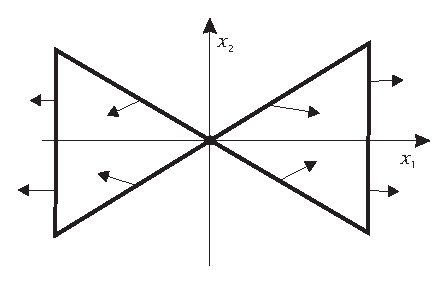
\includegraphics [scale=1.4]{jtr14}
		\caption{Chetaev function.}
		%\vspace{-10pt}
		\label{fig:1.4}
	\end{figure}
	
	To prove these properties, we will use inequalities (which are the consequence of the assumptions made):
	$$\frac{d}{dt} \left|x_1\right| > M\left|x_1\right| - \varepsilon\left|x\right|,\ \frac{d}{dt}\left|x_2\right| < \varepsilon\left|x\right|,$$
	(for $M = \min {\Re \lambda_j: 1 \leq j \leq l}$) and small $\varepsilon$, with the condition that $\left|x\right| < \beta$ ($\beta$ sufficiently small). As usual, $d / dt$ denotes the derivative along the trajectory $x (t)$ of the vector field.
	
	Condition (a) means that $\frac{d}{dt} (\left|x_1\right| - \alpha \left|x_2\right|) |_{\partial_1 V}> 0$. But for $\left|x_1\right| = \alpha \left|x_2\right|$ we have
	$$\frac{d}{dt}(\left|x_1\right| - \alpha \left|x_2\right|) > M\left|x_1\right| - (\alpha+1)\varepsilon \left|x\right| = \left(M - (\alpha+1)^2 \varepsilon \right)\left|x_1\right| >0,$$
	if $\varepsilon$ is small. On the other hand, for $\left|x_2\right|\leq \alpha \left|x_1\right|$ we have
	$$\frac{d}{dt}\left|x_1\right| > (M - (\alpha+1)\varepsilon)\left|x_1\right|>0.$$
	\end{proof}
\end{theorem}

In connection with the above theorems, it raises a natural practical question:

\emph{How to check if all the values of a given matrix have negative real parts?}

Of course this question comes down to the question of the real parts of the roots of the characteristic polynomial of this matrix.

So, let's say we have a polynomial\footnote{The polynomial of $\det(A-\lambda)$ has the coefficient $a_0 = (-1)^n$. Here we take $a_0>0$ to simplify the formulated results.}
\begin{equation}\label{1.6}
	P(\lambda) = a_0\lambda^n + a_1\lambda^{n-1} +  \ldots + a_n, \ a_0>0, \ a_j\in \mathbb{R}.
\end{equation}

\begin{definition}
	We say that the polynomial $P (\lambda)$ is \textbf{stable} if all its zeros $\lambda_j$ have a negative real part, $\Re \lambda_j <0$.
\end{definition}

We ask for the necessary and sufficient conditions for the polynomial \eqref{1.6} to be stable. It turns out that this problem was tested in the 19th century and has a complete solution.

To look at this issue, let us note the following simple necessary condition.

\begin{lemma}
	If the polynomial of the form \eqref{1.6} is stable, then $a_j > 0$ for all $j$.
	\begin{proof}
		Let's look at the factors in the polynomial
		$$P(\lambda) = a_0 \prod (\lambda - \lambda_j) \prod (\lambda^2 -2\alpha_j \lambda + (\alpha_j^2 +\beta_j^2)),$$
		where the first product is related to the real roots $\lambda_j <0$ and the second product is related to the unreal roots $\lambda_j = \alpha_j \pm i\beta_j$, $\alpha_j < 0$, $\beta_j \neq 0$. Since each factor has positive coefficients, then the whole polynomial must also have positive coefficients.
	\end{proof}
\end{lemma}

\begin{remark}\label{remark:1.12}
	If degree $n\leq 2$, then the condition $a_j> 0$, $j = 0, 1, 2$, is also a sufficient condition.
\end{remark}

Let's define the following $n\times n$ dimension matrix:
\begin{equation}\label{1.7}
	M = 
	\begin{pmatrix}
	a_1& a_0 & 0 & 0 & \ldots & 0 & 0\\ 
	a_3& a_2 & a_1 & a_0 & \ldots & 0 & 0\\ 
	a_5& a_4 & a_3 & a_2 & \ldots & 0 & 0\\
	\vdots& \vdots & \vdots & \vdots & \ddots & \vdots & \vdots\\ 
	0& 0 & 0 & 0 & \ldots & a_{n-1} & a_{n-2}\\ 
	0& 0 & 0 & 0 & \ldots & 0 & a_n
	\end{pmatrix}
\end{equation}
such that on the diagonals there are consecutively the numbers $a_1, a_2,\ldots , a_n$. This is called \textbf{Hurwitz matrix}.

\begin{theorem}\emph{(Routh-Hurwitz conditions).} \label{theo:1.13}
	A necessary and sufficient condition for the stability of the polynomial \eqref{1.6} is:
	\begin{enumerate}[(i)]
		\item $a_j > 0$ for all $j$;
		\item the first minors $\Delta_j$ of the matrix \eqref{1.7} are positive.
	\end{enumerate}
\end{theorem}

\begin{example}\label{example:1.14}
	For $n = 1$, the matrix \eqref{1.7} has the form $\begin{pmatrix}
	a_1
	\end{pmatrix}$, so $\Delta_1 = a_1$.
	
	For $n = 2$, that is, the matrix $M = \begin{pmatrix}
	a_1 & a_0\\
	0 & a_2
	\end{pmatrix}$, we have $\Delta_1 = a_1$ and $\Delta_2 = a_2a_1$; therefore, we are under the conditions of Remark \ref{remark:1.12}.
	
	For $n=3$ we have the matrix
	$$\begin{pmatrix}
	a_1 & a_0 & 0\\
	a_3 & a_2 & a_1\\
	0&0&a_3
	\end{pmatrix}.$$
	The Routh-Hurwitz conditions assume the form: $\Delta_1 = a_1> 0$ (nothing new),
	\begin{equation}\label{1.8}
		\Delta_2 = a_1a_2 - a_0a_3 >0
	\end{equation}
	and $\Delta_3 = a_3\Delta_2$ (also nothing new).
\end{example}

\begin{remark}
	It can be shown  that the condition $\Delta_j > 0$ for all $j$ can be replaced by the following Leonard–Shapir condition:
	$$\Delta_2 > 0,\ \Delta_4 > 0,\ \Delta_6 > 0, \ldots$$
	(see also the proof below).
\end{remark}

\begin{proof}[Proof of the Theorem \ref{theo:1.13}]\footnote{The lecture is limited to $n = 3$ and this is required of students on the exam.}
	The idea of proof is quite simple. The condition $\Re\lambda_j < 0$ (and $a_0> 0$) define a certain subset $U$ in the space $\mathbb{R}^{n+1} = \{a\}$ of the coefficients $a_j$. The set $U$ is semi-algebraic and its edge consists of smooth `losses'. It is about equations that define these losses. If you have $a\in\partial U$, then we have two possibilities:
	\begin{enumerate}[(a)]
		\item an element of the equation $P(\lambda) = 0$ is zero,
		\item a pair of complex conjugate roots lies on the imaginary axis.
	\end{enumerate}

Case (a) means that $P (0) = 0$, i.e., $a_n = 0$; this is quite simple.

Let's consider the situation with a pair of $\lambda_{j,j+1} = \pm i\beta$ imaginary elements. We have then
\begin{equation}\label{1.9}
	P_{\beta}(\lambda) = (\lambda^2 + \beta^2)Q(\lambda)
\end{equation}
for a certain polynomial
$$Q = b_0\lambda^{n-2} + b_1\lambda^{n-3} + \ldots + b_{n-2},$$
which we can assume that is stable. In addition, from the inductive assumption (with respect to $n$) we can assume that $b_j> 0$ and the corresponding minor $\Delta_j = \Delta_j(Q) > 0$.

We have the following relationship
$$a_0 = b_0,\ a_1=b_1,\ a_2 = b_2 + \beta^2 b_0,\ a_3 = b_3 + \beta^2b_1, \ldots$$

This means that the matrix $M$ in \eqref{1.7} has to be $M = M_1 + \beta^2M_2$, where
$$M_1 = \begin{pmatrix}
b_1& b_0 & 0 & \ldots & 0  & 0 & 0\\ 
b_3& b_2 & b_1 & \ldots & 0 & 0 & 0\\ 
b_5& b_4 & b_3  & \ldots& 0 & 0 & 0\\
\vdots& \vdots & \vdots  & \ddots& \vdots & \vdots & \vdots\\ 
0& 0 & 0  & \ldots & b_{n-2} & b_{n-3} & b_{n-4}\\ 
0& 0 & 0  & \ldots & 0 & 0 & b_{n-2}\\
0& 0 & 0  & \ldots & 0 & 0 & 0
\end{pmatrix},$$
$$M_2 = \begin{pmatrix}
0 & 0 & 0 & \ldots & 0  & 0 & 0\\ 
b_1& b_0 & 0 & \ldots & 0 & 0 & 0\\ 
b_3& b_2 & b_1  & \ldots& 0 & 0 & 0\\
\vdots& \vdots & \vdots  & \ddots& \vdots & \vdots & \vdots\\ 
0& 0 & 0  & \ldots & b_{n-4} & b_{n-5} & b_{n-6}\\ 
0& 0 & 0  & \ldots & b_{n-2} & b_{n-3} & b_{n-4}\\
0& 0 & 0  & \ldots & 0 & 0 & b_{n-2}
\end{pmatrix}.$$
Let us note that the $r$-th row of the matrix $M_2$ is equal to the $(r-1)$-th row of matrix $M_1$ for $r> 1$. This means that all minors $\Delta_j(P_{\beta})$, $j = 1,\ldots , n - 2$, of the matrix $M$ are equal to the corresponding minor $\Delta_j(Q)$ for the matrix $M_1$ (related to the polynomial $Q$); so they are positive. It follows that $\Delta_{n-1}(P_{\beta}) = 0$ and $\Delta_n(P_{\beta}) = \beta^2b_{n-2} \Delta_{n-1} (P_{\beta}) = 0$.

We can see that the equation $\Delta_{n-1} (P) = 0$ describes locally hyperplanes in the coefficients space ($a_j$) separating the stable polynomials from the unstable. We only have to check if the inequality $\Delta_{n-1} (P_{\beta}) > 0$ locally defines a set of stable polynomials.

For this purpose, we consider the following deformation of the situation \eqref{1.9}:
$$P_{\alpha,\beta} = (\lambda^2 + \alpha^2\lambda + \beta^2)Q(\lambda),$$
where parameter $\alpha$ is small and $\beta$ is real. Then there is another element $\alpha^2M_3$ in the matrix $M$, where in the last two lines of the matrix $M_3$, only the final part of the dimension $2 \times 2$ is non-zero:
$$N = \begin{pmatrix}
b_{n-2} & b_{n-3}\\
0 & 0
\end{pmatrix}.$$
When $\alpha$ and $\beta$ are non-zero, the polynomial $P_{\alpha,\beta}$ is stable; so $\Delta_j(P_{\alpha,\beta})\neq 0$ for $j = 1,\ldots, n - 1$. Let's calculate the boundary $\Delta_{n-1}(P_{\alpha,\beta})$ when $b\to 0$ and constant $\alpha\neq 0$ (then $\Delta_{n}(P_{\alpha,\beta}) \to 0$, because $a_n = \beta^2b_{n-2} \to 0$, but it does not bother us). It is easy to see that for $\beta = 0$ and small non-zero $\alpha$ matrix $M$ takes a block form, with blocks: $M_{11}$ ($(n-2)\times(n-2)$ dimension), $M_{12}$ ($(n-2)\times2$ dimension), $M_{21}=0$ ($2\times(n-2)$ dimension) and $M_{22} = \alpha^2N$. Since $\det M_{11} = \Delta_{n-2}(P_{\alpha,0})$ is close to $\Delta_{n-2}(P_{0,0}) = \Delta_{n-2}(Q) > 0$ (by inductive assumption), so and $\det M_{11}> 0$. Thus
$$\Delta_{n-1}(P_{\alpha,0}) = \det M_{11} \cdot \alpha^2b_{n-2} > 0.$$
\end{proof}

\begin{example}(Watt governor).
	In Figure \ref{fig:1.5}, we have shown a diagram of the Watt governor used in the 19th century in steam engines.This regulator consists of:
	\begin{itemize}
		\item $S$ pin, which can rotate around its axis;
		\begin{figure}[!ht]
			%\vspace{-15pt}
			\centering
			
\includegraphics [scale=1.4]{jtr15}
			\caption{Watt governor.}
			%\vspace{-10pt}
			\label{fig:1.5}
		\end{figure}
		\item two balls of mass $m$ each placed on the movable joints around the pin $S$, so that the upper rim is fixed (merged with $S$) and the lower rim can move up and down (with the balls respectively moving away from the pin and approximating to the pin), furthermore the rods $P_1$ and $P_2$ joining the balls from the upper rim have a length of $l$;
		\item the flywheel $K$ placed on the roll $W$;
		\item a gearbox between the pin $A$ and the roll $W$ at a speed ratio of $n$;
		\item the lever $D$ regulates the steam supply to the machine and is attached to the lower rim.
	\end{itemize}

There are three forces acting on each ball (see Figure \ref{fig:1.6}): mid-force $F_{mid}=ml\theta ^{2}\sin \varphi $ (pointing perpendicular from the pin to the outside), force of gravity $F_{gravity}=mg$ (facing down) and friction $F_{friction}=-b\dot{\varphi}$ (perpendicular to the bars ($P_{1,2}$)). Here $\theta $ is the speed of rotation of the pin $S$ (and balls), $\varphi $ is the angle between the rods $P_{1,2}$ and the pin $S$, $g$ is the acceleration of the earth and $b$ is a coefficient. By summing the components of these forces perpendicular to the rods $P_{1,2}$, we get the following equation of motion
\begin{equation}
\label{1.10}
ml\ddot{\varphi}=ml\theta ^{2}\sin \varphi \cos \varphi -mg\sin \varphi -b \dot{\varphi}.
\end{equation}
This is usually assumed (e.g. in \cite{Pon}), with
$$
l=1,
$$
i.e., in certain units of length.

In equation \eqref{1.10}, in addition to the dynamic variable `there is still a size', which also changes with time. To get any dependency $\theta $ (or its derivatives) from $\varphi $, let's first consider its association
$$
\theta =n\omega
$$
with rotational speed $\omega$ of the cylinder $W$. On the other hand, the motion of the flywheel $K$ is described by the equation
$$
J\dot{\omega}=k\cos \varphi -F,
$$
where $J$ is the moment of inertia of the circle, while on the right we have moment of force acting on the circle. In this case, the component $k\cos \varphi $ is proportional to the amount of steam ($k$ is constant) and $F$ is the constant slowing force due to the work done by the machine. From the above, we consider the following closed and autonomous system of differential equations for $x=\varphi ,$ $y=\dot{\varphi}$ and $z=\omega :$
\begin{equation}
\label{1.11}
\begin{array}{lll}
\dot{x} & = & y, \\
\dot{y} & = & n^{2}z^{2}\sin x\cos x-g\sin x-\frac{b}{m}y, \\
\dot{z} & = & \frac{k}{J}\cos x-\frac{F}{J},%
\end{array}
\end{equation}

\begin{figure}[!ht]
	\centering
	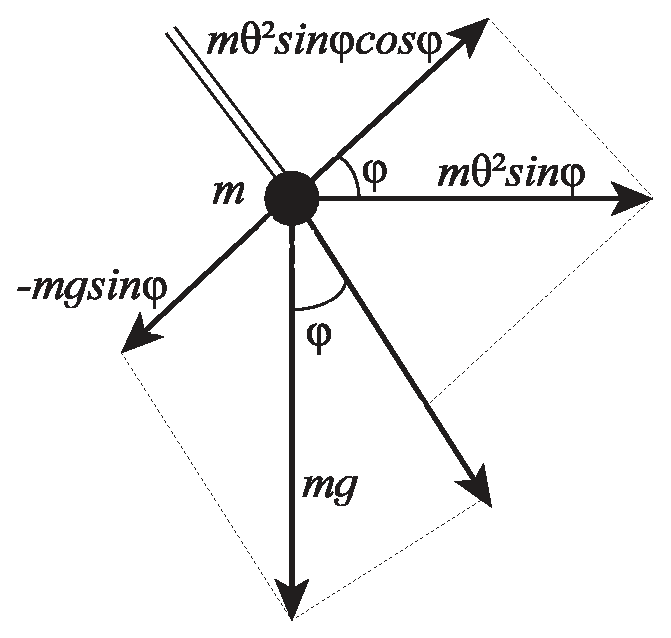
\includegraphics [scale=1]{jtr16}
	\caption{Strength and centrifugal forces.}
	\label{fig:1.6}
\end{figure}

It turns out that this system has exactly one (physically achievable) equilibrium position $(x_{0},y_{0},z_{0})$ given by equations
\begin{equation}
\label{1.12}
\cos x_{0}=F/k,\text{ \ }y_{0}=0,\text{ \ }n^{2}z_{0}^{2}=g/\cos x_{0}.
\end{equation}
In addition, the linearization matrix of the system \eqref{1.11} at this point of equilibrium is the following
\begin{equation}
\label{1.13}
A=
\begin{pmatrix}
0 & 1 & 0 \\
-g\frac{\sin ^{2}x_{0}}{\cos x_{0}} & -\frac{b}{m} & 2g\frac{\sin x_{0}}{%
	z_{0}} \\
-\frac{k}{J}\sin x_{0} & 0 & 0%
\end{pmatrix}
\end{equation}
and its characteristic polynomial is
\begin{equation}
\label{1.14}
\det \left( A-\lambda \right) =-P(\lambda )=-\left\{ \lambda ^{3}+\frac{b}{m}%
\lambda ^{2}+g\frac{\sin ^{2}x_{0}}{\cos x_{0}}\lambda +2kg\frac{\sin
	^{2}x_{0}}{Jz_{0}}\right\} .
\end{equation}

We can see that the coefficients of the polynomial $P(\lambda )$ are positive, that is, the condition (i) of the Routh-Hurwitz theorem. By Example \ref{example:1.14} (for $n = 3$) the condition for sufficient stability of the polynomial $P(\lambda )$ is the inequality \eqref{1.8}, which in this case means
\begin{equation}
\label{1.15}
\frac{bJ}{m}>2k\frac{\cos x_{0}}{z_{0}}=\frac{2F}{z_{0}}
\end{equation}
(Task 1.28). Here $\nu :=z_{0}/2F=\omega _{0}/2F$ has the mechanical interpretation of the \emph{machine unevenness}. So the last inequality is a simple one
$$
\frac{bJ\nu }{m}>1.
$$

The following conclusions can be drawn:
\begin{itemize}
	\item increasing the mass $m$ of the balls aggravates the stability;
	\item decreasing the friction coefficient $b$ aggravates the stability;\footnote{When I presented this example a few years ago at a lecture of Qualitative Theory of ODEs, Z. Nowak informed us about cases where in some German factories (where everything was taken care of) a persistent decrease in the friction coefficient led to the failure of steam engines.}
	\item reducing the moment of inertia $J$ of the flywheel aggravates the stability;
	\item a similar effect is the reduction of the machine's unevenness factor $\nu$.
\end{itemize}	
\end{example}

\section{Hyperbolicity}

The results of the previous chapter have taught us that the condition $\Re \lambda_j = 0$, for a certain value of its own linearization matrix $A$ at the point of equilibrium of the autonomous vector field
\begin{equation}
\label{1.16}
\dot{z}=Az+\ldots ,\text{ \ }z\in \left( \mathbb{R}^{n},0\right) ,
\end{equation}
is a limiting condition for solving asymptotic stability problems of this equilibrium point.
This occurs as follows

\begin{definition}
	An equilibrium point $z = 0$ of the autonomous vector field \eqref{1.16} is called \textbf{hyperbolic point}, if the real parts of all the eigenvalues of its linearization matrix $A$ of the field at this point are non-zero.
\end{definition}

Let us assume that the point $z = 0$ is hyperbolic and consider the corresponding linear system
\begin{equation}
\label{1.17}
\dot{z}=Az.
\end{equation}
Then there is a natural decomposition of the space $\mathbb{R}^n$ on the direct sum of the stable subspace $E^s \simeq \mathbb{R}^k$ and the unstable subspace $E^u \simeq \mathbb{R}^l$, corresponding to the values of $\Re \lambda_j <0$ and $\Re \lambda_j> 0$ respectively:
\begin{equation}
\label{1.18}
\mathbb{R}^{n}=E^{s}\oplus E^{u},\text{ \ \ }A=A_{1}\oplus A_{2}.
\end{equation}
Let us notice that the subspaces of $E^s$ and $E^u$ can be defined topologically in terms of the linear phase flow $g_{Az}^{t}=e^{At}$ of the linear field \eqref{1.17} (see Appendix). Namely,
$$
E^{s}=\left\{ z:g_{Az}^{t}(z)\rightarrow 0,\text{ }t\rightarrow +\infty
\right\} ,\text{ \ }E^{s}=\left\{ z:g_{Az}^{t}(z)\rightarrow 0,\text{ }%
t\rightarrow -\infty \right\}
$$
(see Figure \ref{fig:17}).

\begin{figure}[!ht]
	%\vspace{-15pt}
	\centering
	
\includegraphics [scale=1.4]{jtr17}
	\caption{Hyperbolic saddle.}
	\label{fig:17}
	%\vspace{-10pt}
\end{figure}

It turns out that the analogous situation occurs in the case of the nonlinear field \eqref{1.16}.

\begin{theorem}\emph{(Hadamard-Perron).}\label{theo:1.18}
	For the hyperbolic equilibrium point $z = 0$ of the field $\dot{z} = v (z)$ of class $C^r$, $r> 2$, there exist local submanifolds, stable $W^s$ and unstable $W^u$ of class $C^r$, such that
	\begin{equation}
	\label{1.19}
	W^{s}=\left\{ z:g_{v}^{t}(z)\rightarrow 0,\text{ }t\rightarrow +\infty
	\right\} ,\text{ \ }W^{s}=\left\{ z:g_{v}^{t}(z)\rightarrow 0,\text{ }%
	t\rightarrow -\infty \right\} ,
	\end{equation}
	and\footnote{Here $g_v^t$ denotes the local phase flow generated by the field $v (x)$ and $T_y M$ denotes the tangent space to the manifold $M$ at the point $y$.}
	\begin{equation}
	\label{1.20}
	T_{0}W^{s}=E^{s},\text{ \ \ }T_{0}W^{u}=E^{u}.
	\end{equation}
\end{theorem}
Before we take the proof of this theorem, let us note that analogous concepts and theorems can be introduced for local diffeomorphisms. First, if $z = 0$ is the equilibrium point of the vector field $\dot{z}=v(z)=Az+\ldots$, then $z = 0$ is a \textbf{fixed point} of the flow transformation at time $t = 1$, $f (z) = g^1_v (z)$, i.e.,
$$
f(0)=0.
$$
In addition, the linear part $\frac{\partial f}{\partial z}(z)$ of the transformation $f$ in $z = 0$ has the form of the matrix
$$
\frac{\partial f}{\partial z}(0)=B=e^{A}.
$$
(Task 1.36). In fact, there is a discrete version of the concept of the phase portraits.

\begin{definition}
	The diffeomorphism $f:M\longmapsto M$ defines the homomorphism $\mathbb{Z}\rightarrow \textrm{Diff}(M)$ from the additive group of integers to the group of diffeomorphisms of the manifold so that
	$$
	n\longmapsto f^{n},
	$$
	where $f^{n}=f\circ \ldots \circ f$ ($n$ times for $n \geq 0$) and $f^{-n}=f^{-1}\circ \ldots \circ f^{-1}$ ($\left\vert n\right\vert $ times for $n <0$). In literature $\{f^n\}$ is called \textbf{cascade}.
	
	The point $z_0 \in M$ is a \textbf{periodic point with period} $p \geq 1$ for $f$ if $f^p (z_0) = z_0$; under this we will understand the minimum period (i.e., $f^q (z_0) \neq  z_0$ for $1 \leq q <p$).
	Of course, the periodic point with period $p = 1$ is a fixed point.
\end{definition}

\begin{definition}
	The periodic point $z_0$ of period $p$ of the diffeomorphism $f$ is called \textbf{hyperbolic} if the matrix
	$$
	B=\frac{\partial (f^{p})}{\partial z}(z_{0})
	$$
	has all its eigenvalues outside of a unitary range,
	$$
	\left\vert \lambda _{j}\right\vert \not=1.
	$$
\end{definition}

\begin{lemma}\label{lemma:1.21}
	If $z = 0$ is a hyperbolic equilibrium point for the vector field $v (z)$, then $z = 0$ is also a hyperbolic fixed point of the diffeomorphism $f = g^t_v$, and vice versa \emph{(Task 1.36)}.
\end{lemma}

We have the following version of the Hadamard-Perron theorem for diffeomorphisms.

\begin{theorem}\label{theo:1.22}
	If the fixed point $z=0$ of the local diffeomorphism $f:\left( \mathbb{R}^{n},0\right) \longmapsto
	\left( \mathbb{R}^{n},0\right) $ of class $C^r$, $r \geq 1$, is hyperbolic, there are local subspaces, stable $W^s$ and unstable $W^u$ of class $C^r$, such that
	\begin{equation}
	\label{1.21}
	W^{s}=\left\{ z:f^{n}(z)\rightarrow 0,\text{ }n\rightarrow +\infty \right\} ,%
	\text{ \ }W^{s}=\left\{ z:f^{n}(z)\rightarrow 0,\text{ }n\rightarrow -\infty
	\right\} ,
	\end{equation}
	and
	\begin{equation}
	\label{1.22}
	T_{0}W^{s}=E^{s},\text{ \ \ }T_{0}W^{u}=E^{u},
	\end{equation}
	where $E^s$ and $E^u$ are subspaces of $\mathbb{R}^n$ extracted by their own subspaces corresponding to the eigenvalues of the matrix $B=\frac{\partial f}{\partial z}(0)$ of module $< 1$ and $> 1$ respectively.
\end{theorem}

The path to the proof of the Hadamard-Perron Theorem \ref{theo:1.18} goes through the proof of Theorem \ref{1.22}. 
At the same time, as we shall soon see, the method of proof of the existence of submanifolds $W^s$ and $W^u$ with properties \eqref{1.21} of class $C^0$ is quite natural:
one gets the equation into a fixed point of some transformation in the appropriate infinitely dimensional Banach space.
Unfortunately, `squeezing' the condition of contraction of this transformation is very exhausting.
Therefore, in the following proof we will limit ourselves to deriving the appropriate equations and sketch a general estimation scheme.
For strict proof, we refer the reader to the monograph of W. Szlenk \cite{Szl}.

\begin{proof}[Proof of Theorem \ref{theo:1.22}]
	To simplify the situation, let's assume the decomposition \eqref{1.18}, that is, $\mathbb{R}^{n}=E^{s}\oplus
	E^{u}=\left\{ \left( x,y\right) \right\} $ and the transformation into the form $f=\left( f_{1},f_{2}\right) $, such that
	\begin{equation}
	\label{1.23}
	f_{1}(x,y)=Ax+\varphi (x,y),\text{ \ \ }f_{2}(x,y)=By+\psi (x,y),
	\end{equation}
	where
	\begin{equation}
	\label{1.24}
	\left\Vert A\right\Vert <1,\text{ \ \ \ }\left\Vert B^{-1}\right\Vert <1
	\end{equation}
	and the functions $\varphi $ and $\psi $ are ordered in $O(\left\vert
	x\right\vert +\left\vert y\right\vert )$ (Task 1.37).
	
	Of course, the vector functions $\varphi $ and $\psi $ are defined in a small neighborhood of zero. In the proof, which is presented below, this is a technical obstacle. Therefore, we will make the following change $$
	\varphi \longmapsto \varphi \chi ,\text{ \ \ }\psi \longmapsto \psi \chi ,
	$$ where function $\chi (x,y)$ is smooth (class $C^{\infty }$) and such that:
	\begin{enumerate}[(i)]
		\item $\chi (x,y)\geq 1$ in a small neighborhood of zero, $\left\vert
		x\right\vert +\left\vert y\right\vert <\varepsilon $;
		\item $\chi (x,y)\equiv 0$ outside the small neighborhood of zero, $\left\vert
		x\right\vert +\left\vert y\right\vert >2\varepsilon $ (Task 1.38).
	\end{enumerate}
	Thus, the functions $\varphi \chi $ and $\psi \chi $ after the zero extension for $\left\vert x\right\vert +\left\vert y\right\vert >\varepsilon $ will be determined around $\mathbb{R}^{n}$. Next we mark them with $\varphi $ and $\psi $. Recall that these new functions satisfy $d\varphi (0,0)=0$, $d\psi (0,0)=0$, and $\left\vert \varphi \right\vert $ and $\left\vert \psi \right\vert $ are small with derivatives. By the property (i) the dynamics of the transformation $f$ with the new $\varphi $ and $\psi $ in the zero neighborhood is the same as for the old transformation \eqref{1.23}.
	
	We are looking for a variation of $W^s$ in the form of a graph of a certain mapping (or vector function) $F:E^{s}\longmapsto E^{u}$,
	$$
	W^{s}=\left\{ (x,F(x)):x\in E^{s}\right\} .
	$$
	(Proof of the existence of the $W^{u}$ submanifold is quite similar, so we are confined to the case of $W^{s}$.)
	
	From property \eqref{1.21} it follows that the $W^{s}$ submanifold should be invariant over the diffeomorphism $f,$ $f(W^{s})=W^{s}.$ This means that $f(x,F(x))=(x_{1},F(x_{1}))$ for some $x_{1}\in E^{s}$ depending on $x\in E^{s}$. From \eqref{1.23} we find that $x_{1}=Ax+\varphi (x,F(x)).$ So we get the condition
	$$
	BF(x)+\psi (x,F(x))=F\circ (Ax+\varphi (x,F(x)),
	$$
	that we will write in the following form
	\begin{equation}
	\label{1.25}
	F(x)=B^{-1}\left\{ F\circ (Ax+\varphi (x,F(x))-\psi (x,F(x))\right\} =:%
	\mathcal{T}(F)(x).
	\end{equation}
	We treat the last equation as a fixed point equation $F=%
	\mathcal{T}(F)$ for a nonlinear operator $\mathcal{T}$ defined by the right side of this equality.
	
	Assuming that the functions $ \varphi $ and $ \psi $ are of class $ C^{1} $, it is natural to introduce the Banach space $ \mathcal {X}%
	= C ^ {0} (E ^ {s}, E ^ {u}) $ continuous mapping with supremum norm. It is easy to show that the transformation $ \mathcal {T} $ carries $ \mathcal {X} $ in itself. In order to apply the Banach theorem for constraint mappings, it is still necessary to prove the contradiction condition, they estimate the norm of the difference $ \mathcal {T} (F_ {1}) - \mathcal {T} (F_ {2})$. Here comes the problem, because of (1.25) we get the following inequality:
	$$
	\left\Vert \mathcal{T}(F_{1})-\mathcal{T}(F_{2})\right\Vert
	\leq \left\{ \left\Vert B^{-1}\right\Vert +\left\Vert B^{-1}\right\Vert
	\cdot \left\Vert F_{1}^{\prime }\right\Vert \cdot \left\Vert \varphi
	_{y}^{\prime }\right\Vert +\left\Vert B^{-1}\right\Vert \cdot \left\Vert
	\psi _{y}^{\prime }\right\Vert \right\} \cdot \left\Vert
	F_{1}-F_{2}\right\Vert
	$$
	(Task 1.39). Since $ \left \Vert B ^ {- 1} \right \Vert <1 $ \ (see \eqref{1.24}) and $\left\Vert \psi _{y}^{\prime }\right\Vert =\left\Vert \partial
	\psi /\partial y\right\Vert $ and $\left\Vert \partial \varphi /\partial
	y\right\Vert $ are small (see above), it is only possible to estimate the norm of the derivative $ F_ {1} ^ {\prime} $ mapping $ F_ {1}$. But if we choose $ F_ {1} $ and $ F_ {2} $ arbitrarily from space $ \mathcal {X}$, then  $ F_ {1} $ will only be continuous, and its derivative can be unlimited.
	
	It is out of this deadlock. Let us recall that in the proof of Banach's theorem we choose $ F_ {0} \in \mathcal {X}$, then $ f_ {n} = \mathcal {T} ^ {n} (F_ {0}) $ should converge to a fixed point. The point is to choose the vector function $ F_ {0} $ to show that the functions $ F_ {n} $ are also smooth with appropriately limited norms. It is easy to guess that
	$$
	F_{0}(x)\equiv 0
	$$
	is a good choice. It is also easy to see from formula \eqref{1.24} that $ F_ {n} (x) $  are smooth, e.g. $F_{1}(x)=-B^{-1}\psi (x,0).$
	
	You just have to show that the functions $ F_ {n} (x) $ are uniformly constant. This is reduced to estimate the derivative norm$\left( \mathcal{%
	T(}F)\right) ^{\prime }(x)$ on the assumption, the limits of the norm $ F ^ {\prime} (x)$. We have 
	\begin{equation}
	\label{1.26}
	\left( \mathcal{T(}F)\right) ^{\prime }(x)=B^{-1}\cdot \left\{ F^{\prime
	}\cdot \left[ A+\varphi _{x}^{\prime }+\varphi _{y}^{\prime }\cdot F^{\prime
	}\right] -\psi _{x}^{\prime }-\psi _{y}^{\prime }\cdot F^{\prime }\right\} ,
	\end{equation}
	where we omitted the arguments of the functions appearing on the right side of this equality. Thus the supremum standard is estimated as follows:
	$$
	\left\Vert \left( \mathcal{T(}F)\right) ^{\prime }\right\Vert \leq
	a+b\left\Vert F^{\prime }\right\Vert +c\left\Vert F^{\prime }\right\Vert
	^{2},
	$$
	where $ a $ is small, $ b <1 $ and $ c> 0. $ Hence, if $\left\Vert F^{\prime }\right\Vert $ is small enough, $\left\Vert
	F^{\prime }\right\Vert <d$ (for the appropriate $ d $), then $\left\Vert \left(\mathcal{T(}F)\right) ^{\prime }\right\Vert <d$ (Task 1.40). This gives an even estimate for the norm $ \left \Vert F_ {n} ^ {\prime} \right \Vert $ of the function $ F_ {n}. $
	
	So $ F_ {n} $ converges to the fixed point $ F _ {\ast}$, which we can only say for the time being that it is represented by a continuous mapping of $ E ^ {s} $ to $ E ^ {u } $; that is the submanifold
	$$
	W^{s}=\left\{ (x,F_{\ast }(x))\right\}
	$$
	is of class $ C ^ {0}. $
	
	Let us briefly explain how to measure the smoothness of the function $ F _ {\ast}$. To do this, the equations \eqref{1.25} and \eqref{1.26} must be applied simultaneously to the strings $ \left \{F_ {n} \right \} $ and $\left \{F_ {n} ^ {\prime} \right \} $. In particular, the continuity of the family $ \left \{F_ {n} ^ {\prime} \right \}$, which requires a uniform estimation of the expression
	$\sup \left\vert \left( \mathcal{T(}	F_{n})\right) ^{\prime }(x_{1})-\left( \mathcal{T(}F_{n})\right) ^{\prime}(x_{2})\right\vert $. It turns out that this can be done using the estimates for 
	$\sup \{\left\vert
	F_{n}^{\prime }(x_{1})-F_{n}^{\prime }(x_{2})\right\vert $, $\left\vert
	\varphi ^{\prime }(x_{1},y_{1})-\varphi ^{\prime }(x_{2},y_{2})\right\vert $, $\left\vert \psi ^{\prime }(x_{1},y_{1})-\psi ^{\prime
	}(x_{2},y_{2})\right\vert \}$.

	Then, Ascoli's theorem is used, which says that from a uniformly continuous function on a compact set, one can choose a convergence. Here the compact set is $\left\{ \left\vert x\right\vert <M\right\} \subset E^{s}$ for some $ M $ and the boundary of $ \left \{F_ {n_ {k}} \right \} $ must be $ F _ {\ast} $ (because there is a boundary in the continuous function space).
		
	In this (shortened) proof we limit ourselves to the case where $ f $ is of class $ C ^ {1} $ (and then $ W ^ {s, u} $ are also classes $ C ^ {1}) $. But the case of the class $ C ^ {r} $ for $ r> 1 $ can also be proved by the same method, only the proof requires a larger number of formulas and estimates. We skip it.
	
	Finally, let us note that since $ F_ {0} ^ {\prime} (0) = 0 $ and $ \varphi ^ {\prime} (0,0) = 0 $ and $\psi ^{\prime }(0,0)=0,$ then we have $ F_ {\ast} ^ {\prime} (0) = 0, $ which means that the submanifold $ W ^ {s} $ is tangent to $ \left (0,0 \right) $ to the space $ E ^ {s} $.
\end{proof}

\begin{proof}[Proof of Theorem \ref{theo:1.18}]
	Let us assume $ f = g_ {v} ^ {1}$, that is, transforming the phase flow after time $ t = 1 $ and let $ V ^ {s} $ be a local stable manifold for $ f $ (see Theorem \ref{theo:1.22}). Since the submanifold $ W ^ {s} $ is defined topologically as a set of these points $ z $, that $ g_ {v} ^ {t} (z) \rightarrow 0 $  when $ t \rightarrow \infty$, then $ W ^ {s} \subset V ^ {s} $. On the other hand, if $ z \in V ^ {s} $, then writing $ t = n + \tau $ for $ n \in \mathbb {N} $ and $ 0 \leq \tau <1$, we have $g^{t}(z)=g^{\tau
	}(g^{n}(z))\rightarrow 0$ (as the family $\left\{ g^{\tau }\right\}_{\tau \in \lbrack 0,1)}$ is uniformly continuous).
\end{proof}

The second basic result for hyperbolic fixed points is from D. Grobman and P. Hartman (\cite {Hart}). We formulate it simultaneously for cascades and streams.

\begin{theorem}\emph{(Hartman-Grobman).}\label{theo:1.23}
	Let $f:\left( \mathbb{R}^{n},0\right) \longmapsto \left( \mathbb{R}^{n},0\right) $ be a diffeomorphism of class $C^1$, $r\geq 1$, with a hyperbolic fixed point at $z=0$. Then there is a local homeomorphism $ h: \left (\mathbb {R} ^ {n}, 0 \right) \longmapsto \left( \mathbb{R}^{n},0\right) $ so that
	\begin{equation}
	\label{1.27}
	h\circ f'(0)=f\circ h(z).
	\end{equation}
	
	Analogously, for a local flow $ g_ {v} ^ {t} $ generated by the germ of the vector field $ v \left (z \right)$ with the hyperbolic equilibrium point $ z = 0 $, there is a local homeomorphism $ h $ (as above) that
	\begin{equation}
	\label{1.28}
	h\circ e^{tv^{\prime }(0)}(z)=g_{v}^{t}\circ h(z).
	\end{equation}
	
	\begin{proof}
		Let's start with the cascade case. Similarly to the proof of Theorem \ref{theo:1.22}, we introduce the situation to the case where $ z = \left (x, y \right) $ and
		$$
		f(x,y)=(Ax+\varphi ,By+\psi )=Lz+\tilde{f},
		$$
		where $L=A\oplus B=f^{\prime }(0)$ estimates \eqref{1.24} and $\tilde{f}=\left( \varphi (x,y),\psi (x,y)\right) $ is defined as the whole $ \mathbb {R} ^ {n} = E ^ {s} \oplus E ^ {u} $ and is small with derivatives. Homeomorphism $ h $ will be chosen in the form
		\begin{equation}
		\label{1.29}
		h=id+g=(x+g_{1},y+g_{2}),\text{ \ \ }g\text{\ small.}
		\end{equation}
		
		Equation \eqref{1.27} on $ h $, which denotes the alternation of the following diagram
		$$
		\begin{array}{ccc}
		\mathbb{R}^{n} & \overset{f}{\longmapsto } & \mathbb{R}^{n} \\
		\uparrow h &  & \uparrow h \\
		\mathbb{R}^{n} & \overset{L}{\longmapsto } & \mathbb{R}^{n}%
		\end{array}%
		$$
		leads to equation $\left( id+g\right) \circ L=L (id+g)+\tilde{f} \circ (id+g)$. In the composition we get the system of equations
		$$
		\begin{array}{lll}
		g_{1}(Ax,By) & = & A g_{1}(x,y)+\varphi (x+g_{1},y+g_{2}), \\
		g_{2}(Ax,By) & = & B g_{2}(x,y)+\psi (x+g_{1},y+g_{2}).
		\end{array}
		$$
		Let's rewrite this layout in a convenient way for us
		\begin{equation}
		\label{1.30}
		\begin{array}{lll}
		g_{1}(x,y) & = & A g_{1}(A^{-1}x,B^{-1}y)+\varphi \circ (id+g)\circ
		(A^{-1}x,B^{-1}y), \\
		g_{2}(x,y) & = & B^{-1} g_{2}(Ax,By)-B^{-1}\cdot \psi \circ (id+g).%
		\end{array}
		\end{equation}
		It is easy to recognize here the equation of the fixed point $ g = \mathcal {T} (g) $ for the nonlinear operator $ \mathcal {T} $ acting on $ g = (g_ {1}, g_ {2}) $ by the right hand side of \eqref{1.30}.
		
		We will choose the Banach space
		$$
		\mathcal{X}=C^{0}(\mathbb{R}^{n},E^{s})\oplus C^{0}(\mathbb{R}^{n},E^{u})
		$$
		with norm $\left\Vert g\right\Vert =\sup \left\vert g_{1}\right\vert +\sup
		\left\vert g_{2}\right\vert $. Here it is easy to show that the operator $ \mathcal {T} $ converts a sphere in $ \mathcal {X} $ with a proper radius in itself and is a contraction. The basic argument is that $ A $ and $ B ^ {- 1} $ matrices have a norm $ <1 $.
		
		Let us break away for a moment from our proof and consider the situation when equation \eqref{1.27} is replaced by equation
		\begin{equation}
		\label{1.31}
		k\circ f=L\circ k,
		\end{equation}
		where $k:\mathbb{R}^{n}\longmapsto \mathbb{R}^{n}$. After the substitution $k=id+l=(x+l_{1},y+l_{2})$ and some transformations, we get the following system analogue to \eqref{1.30}:
		$$
		\begin{array}{lll}
		l_{1}(x,y) & = & Al_{1}\circ f^{-1}(x,y)-\varphi \circ f^{-1}(x,y), \\
		l_{2}(x,y) & = & B^{-1}l_{2}(x,y)+B^{-1}\psi (x,y).%
		\end{array}%
		$$
		Here we are dealing with a fixed point equation for the corresponding transformation of $ \mathcal {S}: \mathcal {X} \longmapsto \mathcal {X} $, which is coherent. So also the system \eqref{1.31} has a solution.
		
		Let us note the following property of solutions of equations \eqref{1.27} and \eqref{1.31}, which are the consequence of the fact that in Banach's thesis the fixed point of convergence in the Banach space is constant depending on the parameters (if the transformation itself depends on the parameters continuously):
		
		\emph{The solutions $ h (x, y) $ and $ k (x, y) $ of the equations \eqref{1.27} and \eqref{1.31} are unique and depend in a continuous manner on the data in these equations (i.e. $ L = A \oplus B $ and $ \tilde {f} = (\varphi, \psi)) $. In addition, in equation \eqref{1.27} we can substitute the linear transformation $ L = f ^ {\prime} (0) $ by any transformation $ g $ such that $ g ^ {\prime} (0) = L$.}
		
		The above-mentioned uniqueness will allow us to prove that the transformations $ h $ and $ k $ are homeomorphisms; more precisely, $ h \circ k = k \circ h = id $. In fact, the transformation $ m = k \circ h $ satisfies the condition $ m \circ L = L \circ m$, at equation \eqref{1.27} for $ f = L $. Analogously, the transformations $ n = h \circ k $ and $ id $ satisfies the equation $ f \circ n = n \circ f $.
		
		Let's now take a proof of the second part of the theorem, that is, the homeomorphism of $ h $, which satisfies all of the equations of type \eqref{1.27} for the family of transformations $ f_ {t} = g_ {v} ^ {t}, $ $ v = Az + \ldots $. For each $ t \not = 0 $  the transformation $ f_ {t} $  have the hyperbolic fixed point $ z = 0 $. Thus, from the proved part of the first part of the theorem we have the existence of a family of homeomorphisms $ h_ {t} $, $ t \not = 0 $, such that
		$$
		h_{t}\circ e^{At}=f_{t}\circ h_{t}.
		$$
		We just have to show that $ h_ {t} $ does not depend on $ t $, which we treat here as a parameter. At least we know that $ h_ {t} $ depends on $ t $ in a continuous manner.
		
		Let us now define the following identity
		$$
		h_{t/2}\circ f_{t}\circ h_{t/2}^{-1}=\left( h_{t/2}\circ f_{t/2}\circ
		h_{t/2}^{-1}\right) \circ \left( h_{t/2}\circ f_{t/2}\circ
		h_{t/2}^{-1}\right) =e^{At/2}\circ e^{At/2}=e^{At}
		$$
		(here we used the group property of the phase flow). It means that $ h_ {t / 2} = h_ {t} $ (uniqueness). Similarly it is proved that $ h_ {t / k} = h_ {t} $  for natural $ k $  and hence that
		$$
		h_{kt/l}=h_{t},\text{ \ \ }k,l\in \mathbb{N},
		$$
		(Task 1.41). Let us say that for a measurable set of parameters $ t $ the transformations $ h_ {t} $ are the same. The constant $ h_ {t} $ of the parameter (see above) implies $ h_ {t} \equiv \textrm {const} $ as a function from $ t> 0 $. Now observe that if $ h $ satisfies the equation \eqref{1.28} for a given time $ t> 0$, then this equation for $ -t $ (Task 1.42) ends the proof.
		
		Finally, one more note.	Since $ \left \{g_ {v} ^ {t} \right \} $ is only a local phase potentiometer (for the vector field $ v (z)$ defined in the neighborhood of $ z = 0$) it is necessary to take care of the fields of the transformations of the flow, and thus to the domains of transformations $ h_ {t} $. But there is no problem here because the domain of transformation $ g_ {v} ^ {t / k} $ increases with the increase of $ k \in \mathbb {N} $. Just in the above proof, we limit ourselves to times such that $ \left \vert t \right \vert <1 $.
	\end{proof}
\end{theorem}

Equality \eqref{1.27} means that the dynamics (i.e. cascade) generated by the diffeomorphism $ f $  is the same from the qualitative point of view as the dynamics generated by the linear diffeomorphism $L (z) = f ^ {\prime}(0)z $. Indeed, if $\left\{ \ldots, f^{-1}(z_{0}), z_{0}, f(z_{0}), f^{2}(z_{0}), \ldots \right\} $ is the orbit of the point relative to the diffeomorphism $ f $ and $y_{0}=h(x_{0})$, then $\{\ldots, L^{-1}(y_{0}), y_{0},\linebreak L(y_{0}), \ldots \}$ is the orbit of the point $y_{0}$ relative to the linear diffeomorphism $ L $.

The following definition seems natural.

\begin{definition}\label{def:1.24}
	If for the diffeomorphisms $ f: M \longmapsto M $ and $ g: N \longmapsto N $  there exists a homeomorphism $ h: M \longmapsto N $  such that
	$$
	g=h\circ f\circ h^{-1},
	$$
	we say that the diffeomorphism $ f $ and $ g $ are \textbf {topologically conjugated} (via $ h $). If $ h $ is of class $ C ^ {r} $, then we say that $f$ and $g$ are \textbf{$ C ^ {r} $-conjugated}. Similarly, the vector fields $ v (x) $ and $ w (x) $ are topologically (or classes $ C ^ {r}) $  \textbf{conjugated} if their phase flows are conjugated by a homeomorphism (or diffeomorphism of class $ C ^ {r}) $.
	
	If the diffeomorphism $ f $ has the property that any diffeomorphism $ g $ which is close to $ f $ (in a class that we do not want to emphasize here) is topologically conjugated with $ f $, then we say that $ f $ is \textbf {structurally stable}. Similarly, the vector field $ v (x) $ is \textbf {structurally stable} if the close vector fields are topologically conjugated to it.
\end{definition}

Hartman-Grobman's theorem states that the diffeomorphism (vector field, respectively) in the hyperbolic fixed point (hyperbolic equilibrium point, respectively) is topologically conjugated to the linear part of the diffeomorphism (vector field, respectively). We can prove more.

\begin{proposition}\label{prop:1.25}
	A diffeomorphism (vector field, respectively) in a neighborhood of a hyperbolic fixed point (hyperbolic equilibrium, respectively) is structurally stable.
	\begin{proof}
		We use the following direct construct of the homeomorphism $ h $, which associates two divergent diffeomorphisms $ f $ and $ g $ in the case of the asymptotically stable, i.e., that $ f ^ {\prime} (0) $ and $ g ^ {\prime} (0) $ have all their own values of module $ <1 $. It can be assumed that $ E ^ {s} = \mathbb {R} ^ {n} $ and $ z = x $ in the proof of Hartman-Grobman theorem. Then there is a `Lyapunov function', $ L (x) $, such that satisfies condition (i) of Definition \ref{def:Lyap_funct} and the following analogous condition to (ii):
		$$
		L(f(x))<L(x)\text{ \ for \ }x\not=0.
		$$
		Its construction is exactly the same as in the proof of the Lyapunov Theorem. We can assume that $ L (x) = \left \vert x \right \vert ^ {2} $ in the corresponding (linear) coordinate system. Let $ M (x) = \left \vert x \right \vert ^ {2} $ be the corresponding Lyapunov function for the $ g $ diffeomorphism (also in the corresponding coordinate system). We have two copies of $ \mathbb {R} ^ {n} $, which deal respectively with the diffeomorphisms $ f $ and $ g $.
		
		\begin{figure}[!ht]
			%\vspace{-15pt}
			\centering
			
\includegraphics [scale=1.1]{jtr18}
			\caption{Coupling construction.}
			\label{fig:1.8}
			%\vspace{-10pt}
		\end{figure}	
	Let us take a small $ \varepsilon> 0 $ and consider hyperplanes (diffeomorphic with spheres) $ \left \{L (x) = \varepsilon \right \} $ i $ \left \{M (x) = \varepsilon \right \} $. Let's define the homeomorphism $ h $ between these hyperplanes as $ h|_{L = \varepsilon} = id: \left \{L = \varepsilon \right \} \longmapsto \left \{M = \varepsilon \right \} $ (see Figure \ref{fig:1.8}). Condition 
	\begin{equation}
	\label{1.32}
	h\circ f^{-1}=g^{-1}\circ h
	\end{equation}
	allows us to `transform' $ h $ between the hyperplanes $f(\left\{ L=\varepsilon \right\} )$ and $g\left( \left\{ M=\varepsilon \right\} \right)$, as shown in Figure \ref{fig:1.8}. Let $ h $ be continuous and mutually exclusive to the area between hyperplanes $ \left \{L = \varepsilon \right \} $ and $ f \left (\left \{L = \varepsilon \right \} \right ) $. Using the multiple equation \eqref{1.32} extends us $ h $ to the whole area $ \left \{0 <L \leq \varepsilon \right \} $. By putting $ h (0) = 0 $ we get the desired homeomorphism.
	
	The analogous construction works in the case of extending diffeomorphisms, i.e., when the $ f ^ {\prime} (0) $ and $ g ^ {\prime} (0) $ have their eigenvalues with module $> 1 $.
	
	Let's now consider two linear diffeomorphisms $ f_ {0} $ and $ g_ {0} $ defined by the hyperbolic matrix $ A = A_ {s} \oplus A_ {u} $ and $ B = B_ {s} \oplus B_ {u}$ in the corresponding (and the same) distributions $ \mathbb {R} ^ {n} = E ^ {s} \oplus E ^ {u} $. From the above considerations, we get the homeomorphisms $ h_ {s} $ and $ h_ {u} $, which join $ A_ {s} x $  with $ B_ {s} x $  and $ A_ {u} y $ with  $ B_ {u} y $ respectively. Now, the homeomorphism 
	$$
	h=h_{s}\oplus h_{u}
	$$
	takes $ f_ {0} $ to $ g_ {0}$.
	
	Let's now consider the $ f $ diffeomorphism in the neighborhood of the hyperbolic fixed point $ z = 0 $ and its small disturbance $ g $ with the same fixed point. Since the matrix $B=g^{\prime }(0)$ is close to the matrix $ A = f ^ {\prime} (0) $ is also hyperbolic with the same dimensions of the stable and unstable subspaces; that is, we can apply the above construction of the homomorphic homeomorphism of the linear parts of these diffeomorphisms. We see that $ f $ is conjugated with $ f_ {0} = f ^ {\prime} (0)z $, $ f_ {0} $ is conjugated with $ g_ {0} = g ^ { \prime} (0) z $ and $ g_ {0} $ is conjugated with $ g $; by comparing these three homeomorphisms one gets that $ f $ is conjugated with $ g $.
	
	The case of Proposition \ref{prop:1.25} for vector fields is left to the readers as an exercise (Task 1.43).
	\end{proof}
\end{proposition}

\begin{remark}
	You can ask if Grobman-Hartman's thesis can be strengthened, i.e., if the homeomorphism $ h $ can be of class $ C ^ {1} $. It turns out that no. For example, the transformation $ \left (x, y, z \right) \longmapsto \left (\frac {1} {2} x, 4y, 2z + xy \right) $ can not be linearized using a  $C ^ {1} $-diffeomorphism   (see \cite {Hart}, Problem 8.1). This problem is related to resonances between eigenvalues (see Poincaré Theorem in Chapter \ref{sec:3.3}).
\end{remark}

\subsection*{Tasks}
\begin{task}
	Complete the proof of Lemma \ref{lemma:1.7}, i.e., in case of non-real values.
\end{task}
\begin{task}
	Prove the formulas $(1.11)$ - $(1.15)$.
\end{task}
\begin{task}
	Determine the stability (in Lyapunov and asymptotic terms) for the singular point $ x = d / c $, $ y = a / b $, at the Lotka-Volterra system
	\begin{equation}
	\label{1.33}
	\dot{x}=x(a-by),\text{ \ \ }\dot{y}=y(cx-d),\text{ \ \ }abcd>0,
	\end{equation}
	which describes the dynamics of two competing populations (predators and preys).
	
	Note: Proposition \ref{prop:2.11} below.
\end{task}
\begin{task}
	Using the Definition \ref{def:1.1}, check that the equilibrium point $ x (0) = 0 $ for the equation $ \dot {x} = 4x-t ^ {2} x $ is stable in Lyapunov's sense, i.e., with $ t_ {0} = 0 $.
\end{task}
\begin{task}
	Determine the stability of the equilibrium point $ x = y = 0 $ for the system $ \dot {x} = e ^ {x + 2y} - \cos 3x $, $ \dot {y} = \sqrt {4 + 8x} 2e^ {y} $.
\end{task}
\begin{task}
	Determine the stability of the solution of $ \dot {x} = e ^ {x} -e ^ {3z} $, $ \dot {y} = 4z-3 \sin (x + y) $,  $ \dot { z} = \ln (1 + z-3x) $.
\end{task}
\begin{task}
	For what value of $ a $, the solution of $ \dot {x} = ax + y + x ^ {2} $, $ \dot {y} = x + ay + y ^ {2} $ is asymptotically stable?
	
	Note: When $ a = -1 $, the straight $ y = x $ is invariant.
\end{task}
\begin{task}
	For what parameters of $ a $ and $ b $, the solution of $\dot{x}=y+\sin x$, $\dot{y}=ax+by$ is asymptotically stable?
	
	Note: for $ a = b \leq -1 $, by introducing $ z = \dot {x} $, the system returns into $ \dot {x} = H_ {z} ^ {\prime} $, $ \dot {z} = {H} {x} ^ {\prime} - (a + \cos x) z$, $H=\frac{1}{2}z^{2}-a(\frac{1}{2}x^{2}+1-\cos x)$, and find the Lyapunov function.
\end{task}
\begin{task}
	For what parameters of $ a $ and $ b $, the solution $ x (t) \equiv 0 $ of the equation $ \dddot {x} +3 \ddot {x} + a \dot {x} + bx = 0 $ is asymptotically stable?
\end{task}
\begin{task}
	Show that the diffeomorphism $ g ^ {t} $ (locally) of the phase flow generated by the vector field $ \dot{x}=Ax+O\left( \left\vert x\right\vert ^{2} \right)$ has a linear part at the fixed point $ x = 0 $ of the form $ B = e ^ {At} $. From here, deduce Lemma \ref{lemma:1.21}.
\end{task}
\begin{task}
	Prove the estimates \eqref{1.24} (for the corresponding coordinate system and Euclidean norm in $ \mathbb {R} ^ {n}) $.
\end{task}
\begin{task}
	Give the explicit formula to the function $ \chi $ from proof of Theorem \ref{theo:1.22}.
\end{task}
\begin{task}
	Prove the inequalities for $ \left \Vert \mathcal {T} (F_ {1}) - \mathcal {T} (F_ {2}) \right \Vert $  from proof of Theorem \ref{theo:1.22}.
\end{task}
\begin{task}
	Give a formula for $ d $, depending on $ a, b, c $, in terms of $ \left \Vert (\mathcal {T} (F)) ^ {\prime} \right \Vert <d $.
\end{task}
\begin{task}
	Prove that $h_{\frac{k}{l}t}=h_{t}$ for $ k, l \in \mathbb {N} $ and $ t \not = 0 $.
\end{task}
\begin{task}
	Prove that if $ h $ satisfies property \eqref{1.28} for a given $ t> 0 $ then it also satisfies this property for $ t <0 $.
\end{task}
\begin{task}
	Complete the proof of Proposition \ref{prop:1.25}.
\end{task}